\documentclass{report}
%\usepackage[italian]{babel}
\usepackage{float}
\usepackage{setspace}
\usepackage{graphicx}
\graphicspath{ {./img/} }
\usepackage{wrapfig}
\usepackage{caption}
\usepackage{subcaption}
\usepackage{hyperref}
\usepackage[a-3b]{pdfx}
\usepackage{listings}


\title{Compressione dati: Sostituzione dei volti in video compressi tramite face\_recognition}
\author{Astorino Gianluca \and Calò Raffaella \and  Colucci Daniele \and  Federico Carmine \and Galati Emanuele \and Pappalardo Federica}

\begin{document}

\maketitle

\thispagestyle{empty}
\thispagestyle{empty}
\chapter*{Abstract}
Con l’avanzare della tecnologia la risoluzione dei video tende ad aumentare sempre di più, comportando un aumento delle dimensioni dei file. A tal proposito la compressione video è di fondamentale importanza per poter gestire il traffico video, riducendo i requisiti di spazio di archiviazione e, nel contempo, cercando di mantenere una qualità quanto più ottimale possibile. Per ciò che concerne questo lavoro di progetto, che affronta problematiche relative alla manipolazione dei fotogrammi di un video e alla sostituzione dei volti, è altamente probabile che le dimensioni complessive del video aumentino notevolmente; inoltre l’introduzione di manipolazioni visive solleva importanti questioni etiche e legali. L’implementazione di tecniche di compressione non solo riduce le dimensioni del file, facilitando la gestione del video risultante in termini di spazio di archiviazione, ma svolge anche un ruolo importante nella protezione della privacy.

Il progetto proposto sviluppa un’applicazione in grado di manipolare video attraverso una serie di elaborazioni avanzate. L’approccio adottato è stato quello di implementare tre “moduli”, uno che si occupa dell’estrazione dei fotogrammi dal video e del relativo audio, un altro che si occupa del rilevamento dei volti e della loro sostituzione per ciascun fotogramma, e un altro che si occupa di ricostruire il video con i frame modificati; tutto ciò viene automatizzato in un’unica esecuzione dando in input un video, cosicché il programma restituisca in output il video risultante con i volti sostituiti rispetto a quelli presenti nel file multimediale originale.


\thispagestyle{empty}
\tableofcontents
\thispagestyle{empty}

\chapter{Introduzione}

Con il conseguente aumento della risoluzione dei video, ci troviamo di fronte alla sfida di gestire in modo efficiente il crescente volume di dati video senza compromettere la qualità visiva. Questa problematica è al centro del presente lavoro, che si propone di affrontare le sfide connesse alla manipolazione dei fotogrammi di un video e alla sostituzione dei volti, tenendo conto del fatto che ciò solleva importanti questioni relative alla privacy delle persone coinvolte. In un contesto in cui la condivisione di video può coinvolgere soggetti non consenzienti o situazioni sensibili, la manipolazione dei volti diventa un mezzo essenziale per garantire l’anonimato e la riservatezza.

La compressione video non si limita, dunque, a ridurre le dimensioni dei file per una gestione più efficiente dello spazio di archiviazione, ma svolge un ruolo cruciale per la protezione della privacy individuale. Nel tentativo di affrontare questa sfida, progetti precedenti hanno cercato di implementare soluzioni di manipolazione video mostrando alcune limitazioni. Ad esempio, il progetto “mpeg-scrambling” si è concentrato sulla manipolazione dei video utilizzando lo standard MPEG1, il quale non è più comunemente utilizzato. Limitandosi esclusivamente ai video in tale formato, le sue applicazioni erano ristrette e non allineate alle esigenze dell’ampio spettro di formati video attuali. Inoltre, la mancanza di un adeguato riconoscimento dei volti e la scarsa precisione nell’inserimento delle modifiche visive hanno rappresentato limiti sostanziali. Queste lacune evidenziano l’opportunità di una ricerca più approfondita nel campo della manipolazione video. Nel presente lavoro, ci proponiamo di superare queste limitazioni ampliando la compatibilità dei formati video, migliorando il rilevamento dei volti e perfezionando l’inserimento delle modifiche visive.

\section{Face Recognition}
Gli algoritmi di Face Recognition sono algoritmi con lo scopo di riconoscere i volti presenti in un’immagine. \\
L’algoritmo utilizzato si basa su un metodo chiamato \textit{Histogram of Oriented Gradients}, comunemente detto HOG. \\
Questo algoritmo trasforma le immagini in grayscale, e sostituisce ogni cluster 16x16 di pixel con dei gradienti che mostrano la direzione prevalente del flusso della luminositá dell’immagine. Poiché è utilizzata solo la direzione di questo attributo, le immagini molto chiare o le immagini molto scure avranno approssimativamente lo stesso risultato. \\
L’immagine risultante è confrontata con altre immagini HOG risultanti da dataset creati in precedenza per riconoscere la presenza di volti. \\
Poiché i volti possono essere in diverse posizioni e con diverse espressioni, si tenta di posizionare i punti chiave dei volti sempre nella stessa posizione, utilizzando un metodo chiamato Face Landmark Estimation, il quale si basa sul riconoscimento di 68 punti, detti landmark, presenti su ogni volto, come l’angolo esterno degli occhi e il mento. \\
Il volto rilevato dalla fase precedente è quindi interpolato in maniera tale che i landmark rilevati corrispondano a un pattern predefinito utilizzando solo trasformazioni dette affini, ovvero trasformazioni che non impattano le linee parallele nello spazio. \\
\begin{samepage}
    \begin{figure}[!htb]
    \begin{minipage}{0.48\textwidth}
        \centering
        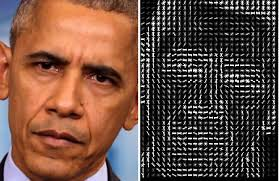
\includegraphics[height=3cm]{hog_obama.jpg}
        \caption{Immagine HOG}
    \end{minipage}\hfill
    \begin{minipage}{0.48\textwidth}
        \centering
        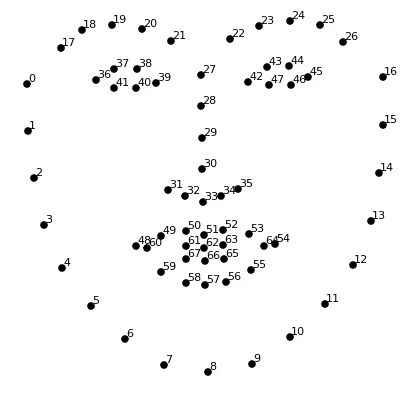
\includegraphics[height=3cm]{landmark.png}
        \caption{Landmark di una faccia}
    \end{minipage}\hfill
    \end{figure}
\end{samepage}
Dopo il riconoscimento dei volti, l’identificazione avviene tramite encoding. Gli encoding di un volto sono una lista di 128 valori ottenuti calcolando la distanza dei diversi landmark. I landmark utilizzati sono risultati di algoritmi di machine learning. Estraendo gli encoding da due volti della stessa persona in immagini differenti, è altamente probabile che le varie misure risultano simili, rendendone quindi possibile l’identificazione. \\

\section{Tecnologie usate}
\subsection{FFmpeg}
FFmpeg permette di leggere e scrivere immagini, video e audio in un ampio numero di formati. Il codec in input è rilevato automaticamente, mentre i video in output utilizzano il codec H.264, molto diffuso e ampiamente supportato per la compressione video ad alta qualità. Per questioni di incompatibilità scaturite dall’impiego del codec in sistemi operativi diversi sono stati utilizzati i codec nativi di FFmpeg, senza fare ricorso a implementazioni esterne.

\subsection{dlib}
Dlib è un moderno toolkit C++ contenente algoritmi e strumenti di apprendimento automatico per la creazione di software complesso in C++ per risolvere problemi del mondo reale. Questa libreria fornisce strumenti per il rilevamento di oggetti nelle immagini, incluso il rilevamento del volto frontale e la stima della posa dell’oggetto, ed un riconoscimento facciale di alta qualità.

\subsection{Python}
E’ stato adottato il linguaggio Python per la semplicitá di implementazione e leggibilitá rispetto ad altri linguaggi come C++, e  per la sua portabilità del codice, dunque programmi scritti in Python possono essere eseguiti su diverse piattaforme senza la necessità di modifiche significative e ciò rappresenta un vantaggio dal momento in cui il lavoro sia stato elaborato da un team, con piattaforme eterogenee.

\subsection{face\_recognition}
Python offre una vasta gamma di librerie e framework, tra cui face\_recognition, che semplificano il processo di sviluppo.
La libreria face\_recognition, costruita sopra la libreria dlib, riduce il lavoro manuale necessario per implementare funzionalità specifiche. Nel caso corrente questa libreria offre funzionalità di alto livello, come il riconoscimento di volti noti in immagini e l’identificazione dei volti, confrontandoli con un dataset dato in input, senza richiedere al programmatore di gestire dettagli di basso livello.

\section{Prerequisiti}
Affinché il programma funzioni è necessario installare sul proprio pc:
\begin{itemize}
    \item
    Python;
    \item
    dlib, una libreria C++ open-source utilizzata da face\_recognition;
    \item
    face\_recognition, una libreria Python basata su dlib, specificamente orientata al riconoscimento facciale;
    \item
    FFmpeg, potente suite di software open-source, nel nostro caso utilizzata per la manipolazione e la compressione/decompressione dei file multimediali.
    \end{itemize}
Per poter eseguire correttamente il programma é stato scritto un file README apposito.

\chapter{Implementazione}
\section{Progettazione}
Il progetto si suddivide in 3 fasi principali:
\begin{enumerate}
  \item
    Inizialmente, il programma utilizza la libreria FFmpeg per decomporre un video in singoli frame, archiviandoli in una specifica cartella. Contestualmente, estrae l'audio associato al video.
  \item
    Successivamente, la libreria face\_recognition e dlib vengono impiegate per identificare e isolare i volti presenti nei frame ottenuti al passo precedente. Questi volti sono poi sostituiti con immagini di volti di immagini “sostitutive”, generando così una serie di frame modificati, che vengono archiviati in una destinazione apposita.
  \item
    Nel passaggio finale, il programma ricostruisce il video originale, utilizzando i frame precedentemente modificati, e reintegra l'audio precedentemente estratto, assicurando la sincronia tra le immagini sostitutive e l'audio; in particolare, ad ogni volto presente nel video, viene applicata l’immagine del volto sostitutivo stabilendo un’associazione “volto\_video”-”volto\_sostitutivo” la quale rimane invariata per tutta la durata del video. L'intero processo di manipolazione del video è orchestrato attraverso l'utilizzo di FFmpeg, garantendo un'efficienza e una coerenza nella qualità del risultato finale.
\end{enumerate}
\section{Implementazione}
Il progetto é stato implementato utilizzando quattro file. Il file Main.py ha lo scopo di prendere in input la directory del file video e un flag opzionale che specifica di effettuare la sostituzione anche ai volti non conosciuti. \\
Nell'esecuzione, le computazioni sono effettuate dai file TryFFMPEG, TrySub e TryRebuild.
\subsection{TryFFMPEG.py}
\begin{lstlisting}[language=Python, breaklines=true]
# Crea una sottocartella per contenere l'audio
output_subfolder = output_folder
os.makedirs(output_subfolder, exist_ok=True)

output_path = os.path.join(output_subfolder, 'audio.mkv')

comando = [
    'ffmpeg',
    '-i', video_input,
    '-vn',  # Specifica che non vuoi video, solo audio
    '-y',
    '-c:a', 'copy',  # Specifica il codec audio per il salvataggio come MP3
    output_path
]

subprocess.run(comando)
\end{lstlisting}
Il metodo estrai\_audio() è autoesplicativo, in quanto il suo compito è quello di creare una cartella in cui immagazzinare l’audio del video che gli viene fornito in input. L’audio è conservato in un file .mkv, un formato container che permette di conservare file multimediali di diversi formati. \\
Il comando da eseguire sarà formato da:
\begin{itemize}
        \item
        il percorso dell'eseguibile di FFmpeg che verrà utilizzato per l'operazione di conversione;
        \item
        l’input del file video, dove video\_input è una variabile che contiene il percorso del file;
  \item
        un flag che specifica di ignorare il video e concentrarsi solo sull'audio;
  \item
        un flag che esplicita di non convertire l’audio, utilizzando il codec originale;
  \item
        il percorso del file di output risultante dopo la conversione.
\end{itemize}

\begin{lstlisting}[language=Python, breaklines=true]
# Estrai l'audio prima di dividere il video
estrai_audio(video_input, output_folder)

# Crea una sottocartella per contenere le immagini
output_subfolder = output_folder
os.makedirs(output_subfolder, exist_ok=True)

# Si dovrebbero eliminare i file gia' presenti nella cartella

output_path = os.path.join(output_subfolder, output_pattern)

comando = [
    'ffmpeg',
    '-i', video_input,
    '-q:v', '2',
    output_path
]

subprocess.run(comando)

\end{lstlisting}
La funzione dividere\_in\_frame() esegue estrai\_audio() e solo successivamente estrae i frame del video in input, creando una cartella per conservare le immagini estratte. \\
Il comando da eseguire, in questo caso, sarà composto da: \\
\begin{itemize}
        \item
        il percorso dell'eseguibile di FFmpeg che verrà utilizzato per l'operazione di conversione;
        \item
        l’input del file video, dove video\_input è una variabile che contiene il percorso del file;
  \item
        un flag che imposta la qualitá video (-q:v) a un valore specifico, per ridurre al minimi la ricompressione dei frame estratti;
  \item
        il percorso della directory dove saranno salvati i frame.
\end{itemize}

È inoltre presente una funzione che prende il framerate del video in input.

\subsection{TrySub.py}

\begin{lstlisting}[language=Python, breaklines=true]
def estrai_volto_da_immagine(volto_da_estrarre_path):
# Carica l'immagine contenente il volto da estrarre
immagine = face_recognition.load_image_file(volto_da_estrarre_path)

# Codifica il volto da estrarre
volto_da_estrarre = face_recognition.load_image_file(volto_da_estrarre_path)
codifica_volto_da_estrarre = face_recognition.face_encodings(volto_da_estrarre)[0]

# Trova tutti i volti nell'immagine
face_locations = face_recognition.face_locations(immagine)
codifiche_volto_immagine = face_recognition.face_encodings(immagine, face_locations)
pil_image = None

for codifica_volto in codifiche_volto_immagine:
    # Confronta la codifica del volto estratto con la codifica del volto dall'immagine
    confronto = face_recognition.compare_faces([codifica_volto_da_estrarre], codifica_volto)

    if confronto[0]:
        # Estrai il volto dall'immagine
        top, right, bottom, left = face_recognition.face_locations(immagine)[0]
        face_image = immagine[top:bottom, left:right]

        # Converti l'array NumPy in un oggetto immagine di PIL
        pil_image = Image.fromarray(face_image)

return pil_image
\end{lstlisting}
La funzione estrai\_volto\_da\_immagine(volto\_da\_estrarre\_path) ha lo scopo di estrarre un volto da un'immagine. Esegue i vari passi per l'estrazione dell'immagine HOG e calcola i landmark e gli encoding per ogni volto trovato nell'immagine. \\

La funzione seguente, esegui\_sostituzione(video\_frame\_folder, training\_folder, sub\_images\_folder, output\_folder, generic\_image\_path = ""), é soddivisibile in diverse parti:

\begin{lstlisting}[language=Python, breaklines=true]
# Crea gli array per i volti conosciuti
training_images_array = []
known_face_encodings = []
known_face_names = []
dir = os.listdir(training_folder)
if len(dir) > 0:
    for filename in dir:
        if filename.endswith(".jpg") or filename.endswith(".png"):
            img = face_recognition.load_image_file(os.path.join(training_folder, filename))
            training_images_array.append(img)
            face_encoding = face_recognition.face_encodings(img)[0]
            known_face_encodings.append(face_encoding)
            face_name = Path(filename).stem
            known_face_names.append(face_name)
\end{lstlisting}
In questa parte sono caricate le immagini dei volti conosciuti e ne sono calcolati gli encoding. I valori sono dunque salvati in un array. Un array parallelo si conserva i nomi (presi dal nome del file dell'immagine).

\begin{lstlisting}[language=Python, breaklines=true]
faces_for_substitution = []
for f in os.listdir(sub_images_folder):
    if f.endswith(".jpg") or f.endswith(".png"):
        faces_for_substitution.append(f)

faces_dictionary = {}
index = 0;
for face_name in known_face_names:
    # Se ci sono piu' facce conosciute che facce per la sostituzione, riutilizza le immagini partendo da 0
    sub_image_path = os.path.join(sub_images_folder, faces_for_substitution[index % len(faces_for_substitution)])
    faces_dictionary[face_name] = estrai_volto_da_immagine(sub_image_path)
    index += 1
\end{lstlisting}
In questa parte ad ogni volto conosciuto è assegnato un volto da utilizzare per la sostituzione tramite un dizionario.

\begin{lstlisting}[language=Python, breaklines=true]
for filename in os.listdir(video_frame_folder):
    if filename.endswith(".jpg") or filename.endswith(".png"):
        image_path = os.path.join(video_frame_folder, filename)
        print(image_path)

        # Load an image with an unknown face
        unknown_image = face_recognition.load_image_file(image_path)

        # Find all the faces and face encodings in the unknown image
        face_locations = face_recognition.face_locations(unknown_image)
        face_encodings = face_recognition.face_encodings(unknown_image, face_locations)

        # Convert the image to a PIL-format image so that we can draw on top of it with the Pillow library
        # See http://pillow.readthedocs.io/ for more about PIL/Pillow
        pil_image = Image.fromarray(unknown_image)
        # Loop through each face found in the unknown image
        for (top, right, bottom, left), face_encoding in zip(face_locations, face_encodings):
            # See if the face is a match for the known face(s)
            name = "Unknown"

            # Necessario per il funzionamento in caso di sostituzione di tutte le facce senza facce da identificare
            if len(known_face_encodings) > 0:
                matches = face_recognition.compare_faces(known_face_encodings, face_encoding)
                face_distances = face_recognition.face_distance(known_face_encodings, face_encoding)
                best_match_index = np.argmin(face_distances)
                if matches[best_match_index]:
                    name = known_face_names[best_match_index]

            print(name)

            # Controlla se la faccia trovata corrisponde a qualcuno da indentificare
            if name in faces_dictionary:
                myimage = faces_dictionary[name]
            # Se la faccia trovata non corrisponde a nessuno e il programma ha arg -a sostituisci con immagine generica
            elif name == "Unknown":
                if(generic_image != None):
                    myimage = generic_image
            else:
                break


            volto_ritagliato = pil_image.crop((left, top, right, bottom))
            volto_ritagliato.convert("RGBA")
            myimage = myimage.resize((volto_ritagliato.size))
            myimage.convert("RGBA")
            volto_ritagliato.paste(myimage)
            pil_image.paste(volto_ritagliato,(left, top, right, bottom))

        file_name = os.path.splitext(os.path.basename(image_path))[0]
        # Crea il percorso per salvare l'immagine modificata
        output_path = os.path.join(output_folder, f"{file_name}_modified.png")
        # You can also save a copy of the new image to disk if you want by uncommenting this line
        pil_image.save(output_path)
        \end{minted}
\end{lstlisting}
Questa parte é la parte principale della sostituzione: per ogni frame del video si effettua il riconoscimento dei volti presenti nel video e si calcolano gli encoding degli eventuali volti. \\
Gli encoding sono successivamente confrontati con i valori estratti in precedenza, per riconoscere se è presente un match tra i due. Se il match è presente, si effettua la sostituzione del volto conosciuto con il volto associato al quel nome nella fase precedente, altrimenti si valuta se è stato impostato il flag di sostituzione dei volti sconosciuti: se è stato impostato, si sostituisce il volto con l'immagine generica, altrimenti si ignora.

\subsection{TryRebuild.py}
Questo file contiene una sola funzione, con lo scopo di ricomporre il video partendo dai frame sostituiti:
\begin{lstlisting}[language=Python, breaklines=true]
frames_path = frames_folder

comando = [
    'ffmpeg',
    '-framerate', framerate,  # Sostituisci con l'fps corretto, da ottenere tramite la funzione get_framerate
    '-i', os.path.join(frames_path, 'frame_\%04d_modified.png'),  # Sostituisci con il pattern corretto
    '-c:v', 'libx264',
    '-c:a', 'copy',
    '-y',
    '-shortest',
    output_path
]

if os.path.exists(audio_file):
    comando += ["-i", audio_file]
\end{lstlisting}
Il comando FFmpeg chiamato sarà formato da:
\begin{itemize}
  \item
        il percorso dell'eseguibile di FFmpeg che verrà utilizzato per l'operazione di conversione;
  \item
        il framerate del video;
  \item
        la directory che contiene i fotogrammi modificati, che utilizzano un pattern numerato per conservare l'ordine;
  \item
        un flag che specifica di utilizzare la compressione basata sullo standard x264;
  \item
        un flag che esplicita di non convertire l’audio, utilizzando il codec originale;
  \item
        un flag che indica di conservare la durata del file piú corto, ovvero l'audio in questo caso;
  \item
        il percorso del file di output risultante dopo la conversione.
\end{itemize}
Se è stato estratto l'audio dal video originale, si aggiunge un altro flag, contenente la directory del file mkv contenente l'audio.

\chapter{Risultati}
I risultati da noi ottenuti hanno portato miglioramenti significativi in confronto al progetto “mpeg-scrambling”, di cui abbiamo parlato in precedenza. \\
Oltre ad avere una migliore precisione nella sostituzione dei volti, scalandolo in base alla dimensione del volto dell’attore, permette la sostituzione di volti di più persone con volti diversi, garantendo l’assegnazione coerente di un volto specifico a ciascuna persona coinvolta. \\

\begin{samepage}
    \begin{figure}[!htb]
    \begin{minipage}{0.48\textwidth}
        \centering
        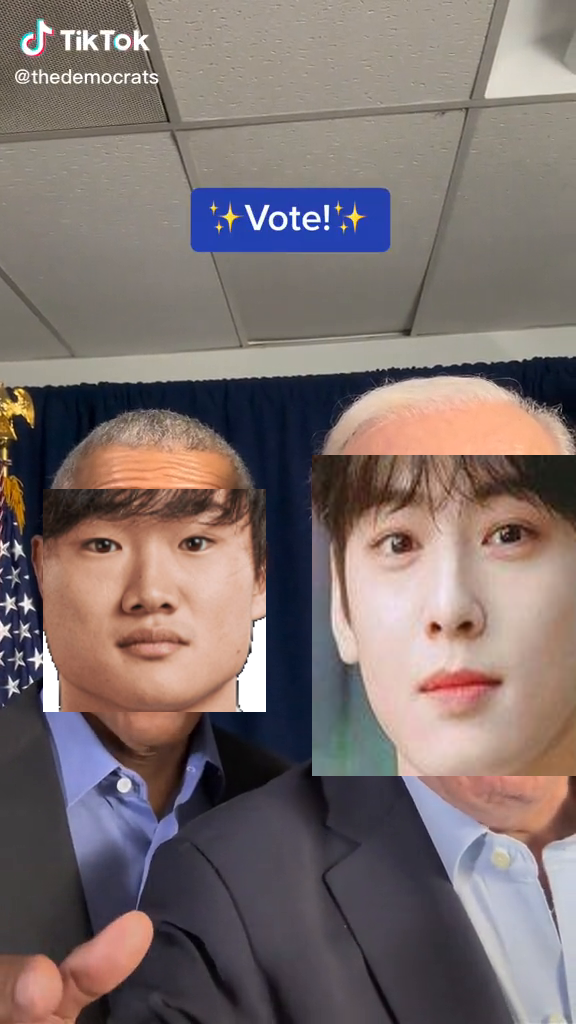
\includegraphics[height=6cm]{frame_obama_biden.png}
    \end{minipage}\hfill
    \begin{minipage}{0.48\textwidth}
        \centering
        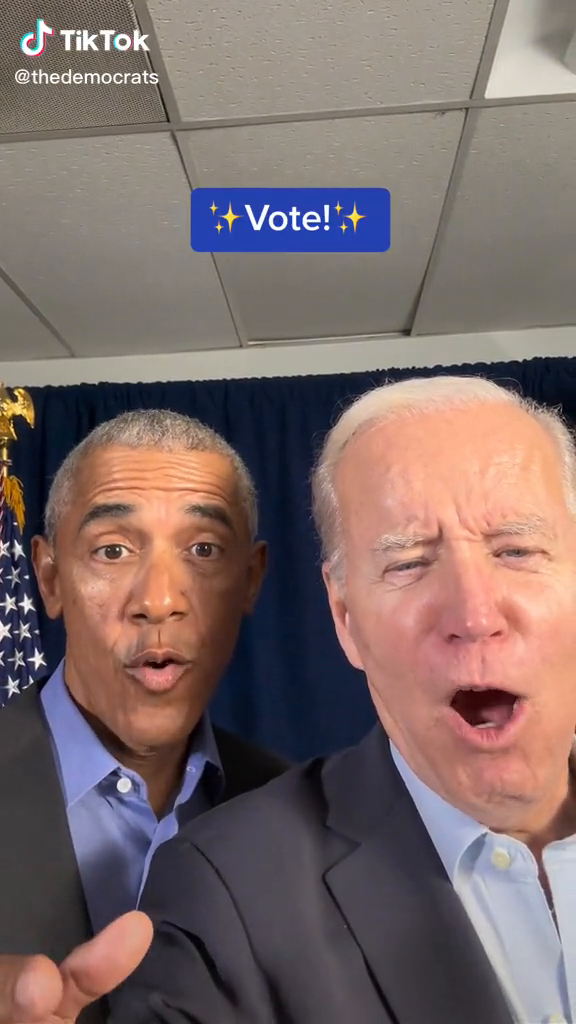
\includegraphics[height=6cm]{frame_obama_biden_sub.png}
    \end{minipage}\hfill
    \end{figure}
\end{samepage}

Nel caso in cui uno o più volti non corrispondono a nessun volto conosciuto, questi saranno ignorati o verranno sostituiti con un’immagine generica se specificato come flag all’avvio.

\begin{samepage}
    \begin{figure}[!htb]
    \begin{minipage}{0.48\textwidth}
        \centering
        
\includegraphics[width=\textwidth]{frame_cena.png}
    \end{minipage}\hfill
    \begin{minipage}{0.48\textwidth}
        \centering
        
\includegraphics[width=\textwidth]{frame_cena_sub.png}
    \end{minipage}\hfill
    \end{figure}
\end{samepage}

Per valutare la qualità del sistema si vedano i tempi di esecuzione del programma su tre video diversi, due dei quali sono stati utilizzati in precedenza nel progetto mpeg-scrambling:

% Tabella
\begin{center}
\begin{tabular}{| c | c | c | c |}
 \hline
 Video & \# Frame estratti & Tempo di esecuzione \\ [0.5ex]
 \hline
 cena.mpg & 250 & 26.197s \\
 \hline
 reporter.mpg & 250 & 58.155s \\
 \hline
 biden\_obama.mp4 & 465 & 4m 26.697s \\
 \hline
\end{tabular}
\end{center}

I tempi di esecuzione includono anche la suddivisione del video in frame e la creazione del video di output, oltre alla sostituzione dei volti. \\
I video cena.mpg e reporter.mpg sono video che seguono lo standard MPEG-1, ad una risoluzione oggi considerata molto bassa. Il video cena.mpg non presenta volti per approssimativamente metá del video, che spiega il suo tempo di esecuzione nettamente minore rispetto agli altri video. \\
Possiamo notare un tempo significativamente maggiore per il video biden\_obama, ciò è dato dalla risoluzione nettamente maggiore del video (576x1024 contro 352x240) e dal fatto che sono presenti i volti di due persone nel training, per questo video il sistema applica il riconoscimento per ciascun frame e quindi si ha un aggravio computazionale. \\
Invece per quanto riguarda gli altri due video, a causa della mancanza dei volti da utilizzare come training, è stata applicata l’immagine di non riconoscimento volto, funzionando quindi come il progetto mpeg-scrambling. \\
\section{Problemi del sistema}
È da sottolineare come il programma non riesca a riconoscere volti parzialmente tagliati o di profilo in maniera soddisfacente: le motivazioni per questo sono date dal funzionamento degli algoritmi utilizzati. \\
È possibile che algoritmi più avanzati riescano a riconoscere i volti in maniera piú soddisfacente, ma il tempo di esecuzione aumenterebbe esponenzialmente senza l’uso di hardware dedicato: un test con l’algoritmo Convolutional Neural Networks, o CNN ha reso il runtime del file cena.mpg ad oltre 14 minuti, ma non ha comunque dato la possibilitá di ottenere precisamente i volti di profilo. \\

\chapter{Conclusioni}
I risultati visti in precedenza hanno dimostrato una buona capacità del sistema di sostituire i volti in video di vari formati in maniera efficace, ciò è dato dalla capacità di adattare il volto da sostituire scalandolo in base al movimento della persona nel video. \\
Ciò che si nota facilmente è l’elevato tempo di esecuzione, che si potrebbe pensare di risolvere in uno sviluppo futuro. \\
Tra i possibili sviluppi futuri si potrebbe anche sostituire il volto, utilizzato da noi come immagine, in maniera più efficace attraverso l’utilizzo di una maschera, data da un insieme di punti tridimensionali, per dare un senso di realismo maggiore. \\

\nocite{*}
\bibliography{citations.bib}
\bibliographystyle{plain}

\end{document}
